%------------------------------------------------------------------------------
% CV in Latex
% Author : Charles Rambo
% Based off of: https://github.com/sb2nov/resume and Jake's Resume on Overleaf
% Most recently updated version may be found at https://github.com/fizixmastr 
% License : MIT
%------------------------------------------------------------------------------

\documentclass[a4paper, 11pt]{article}
%\documentclass[letterpaper,11pt]{article} %For use in US
\usepackage{latexsym}
\usepackage[empty]{fullpage}
\usepackage{titlesec}
\usepackage{marvosym}
\usepackage[usenames,dvipsnames]{color}
\usepackage{verbatim}
\usepackage{enumitem}
\usepackage[hidelinks]{hyperref}
\usepackage[english]{babel}
\usepackage{tabularx}
\usepackage{tikz}
\input{glyphtounicode}

\begin{comment}
I am by no means a professional when it comes to the CV's/resumes, I have
received various trainings on how to write a CV and resume from my high 
school, as well as the Austin College and University of Eastern Finland's
career counseling departments. As I intend to share my CV as a template, I 
feel that it is my responsibility to provide explanations of my work.
\end{comment}


%-----FONT OPTIONS-------------------------------------------------------------
\begin{comment}
The font of the document will impact not just how readable it is, but how it is
perceived. In the "The Craft of Scientific Writing" by Michael Alley, shares a
common fonts for publication as well as their use. I have chosen to use
Palatino for its legibility, some others are given below. There is far too much
about typography to discus here. Note: serif fonts have short projecting
strokes, sans-serif fonts are sans (without) these strokes.
\end{comment}


% serif
 \usepackage{palatino}
% \usepackage{times} %This is the default as well
% \usepackage{charter}

% sans-serif
% \usepackage{helvet}
% \usepackage[sfdefault]{noto-sans}
% \usepackage[default]{sourcesanspro}

%-----PAGE SETUP---------------------------------------------------------------

% Adjust margins
\addtolength{\oddsidemargin}{-1cm}
\addtolength{\evensidemargin}{-1cm}
\addtolength{\textwidth}{2cm}
\addtolength{\topmargin}{-1cm}
\addtolength{\textheight}{2cm}

% Margins for US Letter size
%\addtolength{\oddsidemargin}{-0.5in}
%\addtolength{\evensidemargin}{-0.5in}
%\addtolength{\textwidth}{1in}
%\addtolength{\topmargin}{-.5in}
%\addtolength{\textheight}{1.0in}

\urlstyle{same}

\raggedbottom
\raggedright
\setlength{\tabcolsep}{0cm}

% Sections formatting
\titleformat{\section}{
  \vspace{-4pt}\scshape\raggedright\large
}{}{0em}{}[\color{black}\titlerule \vspace{-5pt}]

% Ensure that .pdf is machine readable/ATS parsable
\pdfgentounicode=1

%-----CUSTOM COMMANDS FOR FORMATTING SECTIONS----------------------------------
\newcommand{\CVItem}[1]{
  \item{
    {#1 \vspace{-2pt}}
  }
}

\newcommand{\CVSubheading}[4]{
  \vspace{-2pt}\item
    \begin{tabular*}{0.97\textwidth}[t]{l@{\extracolsep{\fill}}r}
      \textbf{#1} & #2 \\
      #3 & \ #4 \\
    \end{tabular*}\vspace{-7pt}
}

\newcommand{\CVSubSubheading}[2]{
    \item
    \begin{tabular*}{0.97\textwidth}{l@{\extracolsep{\fill}}r}
      \text{\small#1} & \text{\small #2} \\
    \end{tabular*}\vspace{-7pt}
}

\newcommand{\CVSubItem}[1]{\CVItem{#1}}

\renewcommand\labelitemii{$\vcenter{\hbox{\tiny$\bullet$}}$}

\newcommand{\CVSubHeadingListStart}{\begin{itemize}[leftmargin=0.5cm, label={}]}
% \newcommand{\resumeSubHeadingListStart}{\begin{itemize}[leftmargin=0.15in, label={}]} % Uncomment for US
\newcommand{\CVSubHeadingListEnd}{\end{itemize}}
\newcommand{\CVItemListStart}{\begin{itemize}}
\newcommand{\CVItemListEnd}{\end{itemize}\vspace{-5pt}}

%------------------------------------------------------------------------------
% CV STARTS HERE  %
%------------------------------------------------------------------------------
\begin{document}

%-----HEADING------------------------------------------------------------------
\begin{comment}
In Europe it is common to include a picture of ones self in the CV. Select
which heading appropriate for the document you are creating.
\end{comment}


\begin{minipage}[c]{0.35\textwidth}
\begin{tikzpicture}
    \clip (0,0) circle (1.9cm);
    \node at (0,0) {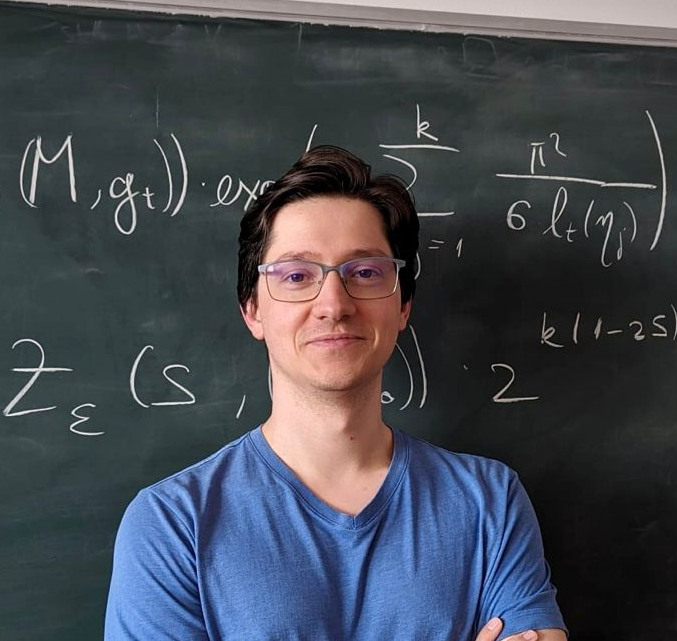
\includegraphics[width = 4cm]{portrait}}; 
    % if necessary the picture may be moved by changing the at (coordinates)
    % width defines the 'zoom' of the picture
\end{tikzpicture}
\hfill\vline\hfill
\end{minipage}
\begin{minipage}[c]{0.6\textwidth}
    \textbf{\LARGE \scshape{Rareș Anghel-Stan}} \\ \vspace{1pt} 
    % \scshape sets small capital letters, remove if desired
    
	+40 769 159 135\\
    Greifswalder Weg, G\" ottingen\\
    \href{mailto:rares1928.de@gmail.com}{rares1928.de@gmail.com}\\
    % Be sure to use a professional *personal* email address
    \href{https://github.com/rares1928}{github.com/rares1928} \\
    \href{https://www.linkedin.com/in/rares-anghel-stan-679340174/}{www.linkedin.com/in/rares-anghel-stan-679340174} \\
    % you should adjust you linked in profile name to be professional and recognizable
    \href{https://www.rares-stan.ro/}{www.rares-stan.ro}
\end{minipage}

% Without picture
%\begin{center}
%    \textbf{\Huge \scshape Charles Rambo} \\ \vspace{1pt} %\scshape sets small capital letters, remove if desired
%    \small +1 123-456-7890 $|$ 
%    \href{mailto:you@provider.com}{\underline{you@provider.com}} $|$\\
%    % Be sure to use a professional *personal* email address
%    \href{https://linkedin.com/in/your-name-here}{\underline{linkedin.com/in/charles-rambo}} $|$
%    % you should adjust you linked in profile name to be professional and recognizable
%    \href{https://github.com/fizixmastr}{\underline{github.com/fizixmastr}}
%\end{center}



\begin{comment}
This CV was written for specifically for positions I was applying for in
academia, and then modified to be a template.

A standard CV is about two pages long where as a resume in the US is one page.
sections can be added and removed here with this in mind. In my experience, 
education, and applicable work experience and skills are the most import things
to include on a resume. For a CV the Europass CV suggests the categories: Work
Experience, Education and Training, Language Skills, Digital Skills,
Communication and Interpersonal Skills, Conferences and Seminars, Creative Works
Driver's License, Hobbies and Interests, Honors and Awards, Management and
Leadership Skills, Networks and Memberships, Organizational Skills, Projects,
Publications, Recommendations, Social and Political Activities, Volunteering.

Your goal is to convey a who, what , when, where, why for every item you share. 
The who is obviously you, but I believe the rest should be done in that order.
For example below. An employer cares most about the degree held and typically 
less about the institution or where it is located (This is still good 
information though). Whatever order you choose be consistent throughout.
\end{comment}

%-----Mission Statement----------------------------------------------------------------
\section{Mission Statement}
As a mathematician with experience as software engineer, I am driven by the pursuit of excellence. My mission is to seamlessly blend analytical rigour with technical proficiency, crafting intelligent solutions to real-world challenges. Leveraging my rich background in mathematics and expertise in software development, I am dedicated to ongoing growth and innovation, aiming to explore new possibilities and expand my skills.

%-----WORK EXPERIENCE----------------------------------------------------------
\begin{comment}
try to briefly explain what you did and why it is relevant to the position you
are seeking
\end{comment}

\section{Work Experience}
  \CVSubHeadingListStart
%    \CVSubheading %Example
%      {What you did}{When you worked there}
%      {Who you worked for}{Where they are located}
%      \CVItemListStart
%        \CVItem{Why it is important to this employer}
%      \CVItemListEnd
    \CVSubheading
      {Software Engineer}{June 2023 -- March 2024}
      {Diomedes-technologies (high-frequency trading firm)}{Bucharest, Romania}
      \CVItemListStart
      	\CVItem{Diomedes ranks amongst the top 50 companies worldwide specializing in cryptocurrency trading.}
        \CVItem{Managed and improved several trading systems, adapting to the unpredictable nature of the trading environment, and regularly tackling new challenges as they emerged.}
        \CVItem{Gained insight into the business operations by visualizing extensive datasets for our research team, utilizing my statistical skills to synthesize the information. This allowed for in-depth analysis of profit and losses, system latencies, and network latencies, thereby enabling informed decision-making and strategic planning.}
        \CVItem{Developed automated processes to streamline data handling for cryptocurrency instruments, resulting in significant time savings and improved data management efficiency.}
        \CVItem{Technical skills: \textbf{Python}, \textbf{SQL}, \textbf{SQLAlchemy}, \textbf{Git}, \textbf{Bash}, \textbf{Grafana}, \textbf{gRPC}, \textbf{ML}.}
      \CVItemListEnd

    \CVSubheading
      {Assistant Researcher}{December 2021 -- Present}
      {Mathematics Institute of the Romanian Academy}{Bucharest, Romania}
      \CVItemListStart
        \CVItem{The Mathematics Institute of the Romanian Academy is the leading mathematical institution in Romania, ranking amongst the top 3 research institutions at the national level.}
        \CVItem{Publications:}
        \begin{itemize}
	        \item[-] \emph{The Selberg trace formula for spin Dirac operators on degenerating hyperbolic surfaces}, \href{https://arxiv.org/abs/2212.11793}{arxiv.org/abs/2212.11793}, to appear in: \textbf{Documenta Mathematica} (ranks amongst top 15\% Mathematical journals worldwide).
	        \item[-] \emph{Spectral convergence of the Dirac operator on typical hyperbolic surfaces of high genus} (with Laura Monk), \href{https://arxiv.org/abs/2307.01074}{arxiv.org/abs/2307.01074}, to appear in: \textbf{Annales Henri Poincaré} (ranks amongst top 20\% Mathematical Physics journals worldwide).
        	\item[-] \emph{Uniformization of Riemann surfaces revisited} (with Cipriana Anghel), \href{https://arxiv.org/abs/2008.12189}{arxiv.org/abs/2008.12189}, \textbf{Annals of Global Analysis and Geometry} (ranks amongst top 40\% Mathematical journals worldwide).
        \end{itemize}
        \CVItem{Selected invited talks:}
        \begin{itemize}
        	\item[-] \emph{The Selberg trace formula for spin Dirac operators on degenerating hyperbolic surfaces}, Geometry and Topology Oberseminar, University of Göttingen, 2023.
    		\item[-] \emph{The uniformization theorem}, Analysis Reading Group seminar, University of Bristol, 2023.
    		\item[-] \emph{The Selberg trace formula for spin Dirac operators}, Geometric seminar, University of Regensburg, 2022.
        \end{itemize}
        \CVItem{Conferences and summer schools:}
        \begin{itemize}
	    		\item[-] Random walks and related random topics, G\" ottingen, 2022.
    			\item[-] Geometry and Analysis on Non-Compact Manifolds, CIRM, Marseille, 2022.
    			\item[-] Heidelberg Laureate Forum, 2018 (I was selected amongst 200 young researchers to spend a week with the recipients of the Abel Prize, Turing Award, ACM Prize, and Fields Medal).
    		\end{itemize}
    	\CVItem{Organized a semester seminar with over 14 meetings providing a self-contained introduction to \textbf{Brownian motion} and the \textbf{Black-Scholes equation}, with a focus on their applications to finance.}
		\CVItem{Teaching assistant for the courses \textbf{Real Analysis} and \textbf{Riemann Surfaces} at University of Bucharest.}
      \CVItemListEnd
  \CVSubHeadingListEnd

%-----EDUCATION----------------------------------------------------------------
\section{Education}
  \CVSubHeadingListStart
%    \CVSubheading % Example
%      {Degree Achieved}{Years of Study}
%      {Institution of Study}{Where it is located}
    \CVSubheading
      {PhD, Mathematics}{November 2019 -- Present}
      {Mathematics Institute of the Romanian Academy}{Bucharest, Romania}

Thesis title: Spectral and algebraic methods in the study of differential manifolds.\\
Expected defense date: \textbf{June 2024}.
    \CVSubheading
      {Master Degree, Mathematics}{October 2017 -- July 2019}
      {University of Bucharest -- Department of Mathematics and Computer Science}{Bucharest, Romania}
      
Graduated with grade 9.75/10 ranking amongst top 3\% of all students.
    \CVSubheading
      {Bachelor's Degree, Mathematics}{October 2014 -- July 2017}
      {University of Bucharest -- Department of Mathematics and Computer Science}{Bucharest, Romania}
      
Graduated with grade 10/10.
  \CVSubHeadingListEnd


%-----PROJECTS----------------------------------------------------
\begin{comment}
Ideally the title of the work should speak for what it is. However if you feel
like you should explain more about why the project is applicable to this job,
use item list as is shown in the work experience section.
\experienceItem[
		company={ReziGo (e-learning platform)},
		location={Bucharest},
		position={Software developer},
		duration={Jan 2020 – Dec 2021}
		]
		\begin{itemize}
			\itemsep -6pt {}
			\item Co-managed a 5 members team  (product, engineering, sales) to successfully launch a website for medical school graduates in Romania to practice for their final exam, attracting about 1000 users annually.
			\item Developed the front-end using \textbf{React} and the \textbf{Material-UI} library, resulting in a modern and user-friendly interface.
			\item Developed the back-end in \textbf{C\#} utilizing \textbf{Azure Functions} for a serverless architecture. Integrated \textbf{Stripe} for payment processing, resulting in over 100 successful payments to date.
		\end{itemize}
\end{comment}

\section{Personal Projects}
  \CVSubHeadingListStart
%    \CVSubheading
%      {Title of Work}{When it was done}
%      {Institution you worked with}{unused}
    \CVSubheading
      {Developed an e-learning platform (\href{https://rezigo.ro}{rezigo.ro})}{January 2020 -- December 2021}
		{Frontend code: \href{https://github.com/rares1928/rezigo_v2}{github.com/rares1928/rezigo\_v2}}{}
      \CVItemListStart
      \CVItem{Co-managed a team of five members, playing a key role in the successful launch of a website tailored for medical school graduates in Romania to prepare for their final exams, attracting approximately 1000 users annually. Played a major role in the development of the website and in the integration of the payment process, resulting in over 100 successful payments to-date.}
      \CVItem{Technical skills: \textbf{JavaScript}, \textbf{Git}, \textbf{React}, \textbf{SQL}, \textbf{CSS}, \textbf{C\#}, \textbf{Stripe}.}
      \CVItemListEnd
  \CVSubHeadingListEnd


%-----HONORS AND AWARDS--------------------------------------------------------
\section{Honors and Awards}
  \CVSubHeadingListStart
%    \CVSubheading %Example
%      {What}{When}
%      {Short Description}{}
    \CVSubheading
      {Bitdefender Scholarship}{2020}
      {Merit based scholarship awarded to two PhD students at the Mathematics Institute.}{}
      \CVSubheading
      {Anghelescu Scholarship}{2017}
      {Recognition for up to 3 students at University of Bucharest -- Department of Mathematics.}{}
      \CVSubheading
      {Bronze medal at IMC}{2016}
      {International Mathematics Competition
for University Students.}{}
    \CVSubheading
      {Silver medal at SEEMOUS}{2016}
      {South Eastern European Mathematical Competition for University Students.}{}
    \CVSubheading
      {Gold medal at the Romanian Mathematical Olympiad}{2014}
      {National level Mathematical Olympiad.}{}

  \CVSubHeadingListEnd



%-----SKILLS-------------------------------------------------------------------
\begin{comment}
This section is compressed from the various skills sections that Euro CV
recommends.
\end{comment}

\section{Skills and Languages}
 \begin{itemize}[leftmargin=0.5cm, label={}]
    {\item{
     \textbf{Languages}{: Romanian (Native), English (C1), German (A2), French (A1).} \\
     \textbf{Programming}{: Python, SQL, Javascript, C\#, R, MATLAB, Mathematica.} \\
     \textbf{Document Creation}{: Microsoft Office Suite, LaTeX, Markdown.} \\
    }}
 \end{itemize}
 
%-----HOBBIES AND OTHER ACTIVITIES-------------------------------------------------------------------
\begin{comment}
This section is compressed from the various skills sections that Euro CV
recommends.
\end{comment}

\section{Hobbies and other activities}
\begin{itemize}[leftmargin=0.5cm, label={}]
\item{
Organizing a book club (\href{https://www.rares-stan.ro/book-club}{www.rares-stan.ro/book-club}), playing Chess, Hiking.}
\end{itemize}
 
    
%------------------------------------------------------------------------------
\end{document}